\documentclass{article}

\usepackage[main,final]{neurips_2026}

\usepackage[utf8]{inputenc}
\usepackage[T1]{fontenc}
\usepackage{hyperref}
\hypersetup{pdftitle={Controller Improvement or Simulator Artifact? Held-Out Evaluation of One-Step MPC for HVAC},pdfauthor={Karmanya Iyer}}
\usepackage{url}
\usepackage{booktabs}
\usepackage{amsfonts}
\usepackage{amsmath}
\usepackage{nicefrac}
\usepackage{microtype}
\usepackage[table]{xcolor}
\usepackage{graphicx}

\newcommand{\TBD}[1]{\textcolor{red}{[#1]}}

\title{Controller Improvement or Simulator Artifact?\\ Held-Out Evaluation of One-Step MPC for HVAC}

\author{%
  Karmanya Iyer \\
  Independent Researcher \\
  \texttt{contact@karmanyaiyer.com} \\
}

\begin{document}

\maketitle

\begin{abstract}
\input{abstract.txt}
\end{abstract}

\section{Introduction}

The Smart Buildings Challenge~\citep{goldfeder2026smart} asks for a single HVAC control policy that is scored on buildings and climates it has never seen. Each policy drives a procedurally generated multi-zone office building in the SBsim simulator~\citep{goldfeder2024smart} for 30 days at 5-minute steps and is scored on a weighted sum of occupant comfort regret, energy cost and carbon emissions. Six training buildings are public. The development leaderboard is computed on 30 scenarios that pair six hidden buildings with five hidden weather stations, and the final round will be re-run on a corrected simulator with a fresh random seed. Development-leaderboard rank is therefore a noisy signal for the final round: it rests on six buildings, and, as participants discussed openly, it rewards behavior that exploits simulator artifacts the organizers have said they will fix before the final evaluation.

We ask which improvements hold up once both problems are removed, and make three contributions.
\begin{enumerate}
  \item \textbf{A held-out, physics-corrected evaluation protocol.} We generate eight new buildings with the official generator, rescaled into the size range of the public buildings, pair them with weather months that no public scenario uses, and evaluate on a simulator with two community-proposed fixes applied (an energy-balanced hot-water tank and airflow-weighted return air). Code, simulator patches and per-scenario results are released at \url{https://github.com/KarmanyaIyer/sb26-heldout-hvac}.
  \item \textbf{A sensitivity analysis of the strongest public controller we found.} We derive the reward's marginal price of gas relative to electricity, watt for watt (0.48 to 0.55, versus 0.30 in the public controller) and find that correcting it barely changes the score: over the settings and states we tested, comfort constraints and plant limits, not cost weights, determine the chosen action. Three small changes (sharper start-up before occupancy, a 2-hour instead of a 72-hour hot-water hold, and a lower unoccupied cooling ceiling) improve the held-out score by 0.27\% on the corrected simulator but worsen it by 7.1\% on the shipped one. On the 30 public scenarios the full set is 0.44\% worse, because the lower ceiling costs up to 4.9\% in hot Phoenix episodes that val16 under-samples; without it, the other two changes improve the score by 0.19\%.
  \item \textbf{Measurements of the value of occupancy information and of simulator artifacts.} Analysis-only oracles that read the simulator's occupancy model improve on the public controller by 5 to 7\%; a test for the 70\,W per-occupant heat gain in the controller's model residual detects nothing; and a simple tank-sawtooth rule gains 7\% on the shipped simulator and under 0.5\% after the fix. These are measured gains of specific policies, not upper bounds on what the information or the artifacts are worth.
\end{enumerate}

\section{Related work}

\paragraph{Benchmark and challenge.} SBsim~\citep{goldfeder2024smart} is an open-source, Gym-compatible suite for evaluating HVAC control policies that generalize across buildings, combining real data from 11 buildings, a lightweight physical simulator and a physics-informed neural building model. The Smart Buildings Challenge~\citep{goldfeder2026smart} builds on it with a procedural building generator (2 to 4 floors, at most 10 zones per air handler, randomized envelope properties and occupancy), a three-term regret reward, and evaluation on six unseen buildings at five unseen weather stations. The challenge paper provides four reference controllers (bang-bang, fixed setpoint, PID and a PID with hot-water reset); we compare against the strongest of these. Other building-control benchmarks, such as BOPTEST~\citep{blum2021boptest}, Sinergym~\citep{jimenez2021sinergym} and CityLearn~\citep{vazquez2019citylearn}, evaluate controllers on fixed, detailed building models or on districts; the challenge instead tests generalization to procedurally generated buildings.

\paragraph{Model-predictive and supervisory HVAC control.} Model-predictive control (MPC) with weather forecasts can cut building energy use substantially relative to rule-based control when a usable thermal model is available~\citep{oldewurtel2012use}; \citet{drgona2020all} survey the modeling, estimation and deployment issues, chief among them the cost of obtaining a model for each new building. Production sequences such as ASHRAE Guideline~36~\citep{ashrae2018g36} instead use supervisory resets (supply-air temperature, duct static pressure, hot-water temperature and pump pressure reset by zone demand) and optimal start from setback. Deep reinforcement learning has also been applied to HVAC control~\citep{wei2017deep}, but transferring a learned policy across buildings is the difficulty the challenge tests. Occupancy can be estimated from environmental signals such as CO$_2$, temperature and light~\citep{candanedo2016accurate}; of these, the challenge observation provides only temperatures, plus a building-wide head count. The controllers we study sit between the MPC and supervisory families: a one-step MPC with a per-zone model identified online during each episode, wrapped in Guideline-36-style supervisory logic.

\paragraph{Public controllers in this challenge.} We start from a chain of public controllers on the challenge's Kaggle forum: a one-step MPC with online per-zone thermal identification and observation-delay compensation by Daniel Wu~\citep{wu2026cpu} (the \emph{base controller}), extended with supervisory refinements (warm standby, weekend hot-water hold, fast recovery, demand-sized hot-water pressure) in a later notebook~\citep{penguin2026} (the \emph{public chain}). Both were shared under the competition's open-source code-sharing rule; we credit both in our code and report both as baselines.

\section{Problem setup}

\paragraph{Reward and metric.} At each step $t$ the environment returns
\begin{equation}
  r_t = 0.6\,p_t - 0.2\,\frac{C^{\mathrm{el}}_t + C^{\mathrm{gas}}_t}{\bar C^{\mathrm{el}}_t + \bar C^{\mathrm{gas}}_t} - 0.2\,\frac{G^{\mathrm{el}}_t + G^{\mathrm{gas}}_t}{\bar G^{\mathrm{el}}_t + \bar G^{\mathrm{gas}}_t},
\end{equation}
where $p_t \le 0$ is occupancy-weighted productivity regret (linear up to 5\,K outside the comfort band, then quadratic and unbounded), $C$ and $G$ are energy cost and carbon, and the bars denote the same quantities evaluated at nominal maximum rates of 80\,kW electricity and 205\,kW gas per air handler. The score of a policy is the mean over scenarios of $-\frac{1}{T}\sum_t r_t$ with $T=8640$ in our harness (the Kaggle gateway executes one extra step); lower is better.

\paragraph{Plant.} Each building has $K$ air handlers (AHUs) serving variable-air-volume (VAV) zones with hot-water reheat from a gas boiler and storage tank. AHUs can only cool (supply air is the minimum of the mixed-air temperature and the setpoint), so all heating comes from VAV reheat. The action space sets per-AHU supply-air temperature, static pressure and run state, and the plant's hot-water supply temperature and pump differential pressure. Zone temperature observations are delayed by one step.

\section{Held-out, physics-corrected evaluation}
\label{sec:protocol}

\paragraph{Why not the public scenarios.} The 30 public scenarios use six buildings, and the leaderboard uses six others. The challenge is about that shift, so a controller tuned on the public buildings has to be evaluated on buildings it was not tuned on. The leaderboard gives too little feedback for this: five submissions per day, each taking up to nine hours to score.

\paragraph{val16.} We ran the official floor and scenario generators from seed 600 upward. The generator's default footprint (400 to 700\,m wide) produces buildings much larger than the public ones, so we rescaled footprints into the public range (width 318 to 430\,m, height 188 to 301\,m) and kept the first eight seeds that pass the generator's own minimum-zone check (seeds 600 and 603 fail). Each building is paired with two weather strips from station months that no public scenario uses, giving 16 scenarios across Fairbanks, Minneapolis, Denver, Atlanta, Phoenix and Singapore (Appendix~\ref{app:val16}). Five of these six stations also appear in the public scenarios, with different months; only Minneapolis is new, whereas all leaderboard stations are unseen.

\paragraph{Corrected simulator.} Two open community pull requests on the official starter kit fix simulator artifacts. First, the hot-water tank billed gas at the boiler setpoint rather than by energy balance, so a sawtooth tank temperature produced unbilled heat; the organizers acknowledged this and asked participants to keep controllers physically consistent. Second, return air was mixed by floor area rather than by airflow. Both of our simulators are built from starter-kit commit \texttt{95cea5b}; the \emph{corrected} simulator adds both pull requests, which we release as a single patch, and the \emph{shipped} simulator has neither. We treat the corrected simulator as primary and the shipped one as secondary. Because the corrected simulator changes two things at once, differences between the two are not attributable to the tank alone.

\paragraph{Fidelity of the harness.} Our rollout harness uses the same scenario loader, metadata builder and occupancy normalization as the Kaggle gateway, and records the three reward terms separately. On public scenario building\_train\_1/atlanta\_2 with the shipped simulator, the Kaggle gateway's commit run of our first submission reported a total reward of $-23.47598$ over 8641 steps and our harness $-23.47109$ over 8640 steps. The difference ($-0.0049$, less than two average steps' reward) is consistent with the gateway executing one extra step; we compared totals, not step-by-step trajectories.

\section{Method}

\subsection{Base controller}
The base controller~\citep{wu2026cpu} keeps, for every zone $i$, a linear one-step temperature model
\begin{equation}
  T_i^{t+1} - T_i^{t} = \theta_i^\top \phi_i^t + \beta_i\, Q_i^t + \epsilon_i^t,
\end{equation}
where $\phi$ contains a bias, the outdoor-to-zone and slow-mode-to-zone temperature differences, the difference to the area-weighted mean of the zone's AHU group, and the comfort-mode flag; $Q_i^t$ is the heat delivered by supply air and reheat; and $\epsilon$ is tracked by an exponentially smoothed residual. Parameters start from a prior computed from the building metadata and are refined online by box-constrained recursive least squares (forgetting factor 0.997, $\beta_i$ kept within $\pm50\%$ of its prior), so nothing is learned offline and nothing is building-specific. Because zone temperatures are observed one step late, the model is rolled forward one step from the last applied action before deciding.

At each step and for each AHU, the controller enumerates a grid of supply-air setpoints (0.5\,K spacing) and recirculation levels, inverts the zone model to find the airflow and reheat that would bring each zone into its target band at the next step, sizes duct static pressure for the most demanding zone, and scores each candidate by
\begin{equation}
  J = P_{\mathrm{fan}} + P_{\mathrm{chiller}} + \lambda_{\mathrm{gas}} Q_{\mathrm{reheat}} + c \sum_i \left(v_i + 2 v_i^2\right),
\end{equation}
where $v_i$ is the predicted band violation in kelvin and $c$ is a comfort price. An ``off'' candidate is chosen when thermal inertia alone keeps all zones in band. The target band is the comfort band (plus a margin that shrinks for zones whose model error is small) during comfort hours and the hour before them, and a wide standby band (274 to 307\,K) otherwise.

On top of this, the public chain~\citep{penguin2026} adds supervisory rules for the hot-water plant: holding the water setpoint warm for 72 hours after the last heat demand (36 hours in an intermediate version) so that the tank stays hot overnight and across weekends, sizing the water temperature to the reheat duty with a 320\,K floor, and running the pump at 0.1\% above the minimum feasible valve pressure. It also relaxes the band on days when the building-wide occupancy count stays at zero. In our runs the controller took 3 to 8\,ms per step and the simulator 90 to 350\,ms (shared machine under parallel load).

\subsection{Reward-consistent fuel weighting}
The controller's per-step objective prices electricity (fan and chiller, in watts) and reheat gas (in watts of heat) with a single ratio $\lambda_{\mathrm{gas}}$. The reward determines what this ratio should be: differentiating $r_t$ with respect to one extra watt of each fuel gives a marginal price per watt per AHU of $2.07$ to $2.25\times10^{-6}$ for electricity and $1.07$ to $1.14\times10^{-6}$ for gas, so $\lambda_{\mathrm{gas}} \in [0.48, 0.55]$ depending on the hour (time-of-use electricity prices). The boiler model has unit efficiency, so a watt of reheat is a watt of gas. The public controller uses $\lambda_{\mathrm{gas}} = 0.30$, which under-prices heat by roughly 40\%. Yet correcting it barely changes the score (Section~\ref{sec:results}). A plausible explanation, which our decision probe supports but does not prove, is structural. When a zone needs heat, every useful candidate delivers the heat needed to reach the band edge; the one with the warmest supply air (maximum recirculation, highest setpoint the mixed air allows) needs the least airflow and therefore the least fan power and outdoor-air reheat, so it is preferred across a wide range of $\lambda_{\mathrm{gas}}$. Likewise, the comfort price is large relative to the energy terms, so candidates with a predicted violation rarely win. Cost weights in a one-step search of this kind matter mainly where candidates trade one fuel against another at equal comfort, a choice this plant seldom offers. We nonetheless use $\lambda_{\mathrm{gas}}=0.5$ in all of our variants.

\subsection{Sharper start-up before occupancy}
The observation includes a flag that turns on 60 minutes before comfort hours, and the public chain applies the comfort band only while that flag or comfort mode is set. We decode weekday and hour from the cyclic time features, compute the time $h$ until the next weekday comfort period, and hold zone $i$ to the comfort band with the full comfort margin whenever $h \le \min(\ell_0 + \ell_1 \Delta_i, \bar\ell)$, where $\Delta_i$ is the zone's current deficit from the band in kelvin. We use $\ell_0 = 0.25$\,h, $\ell_1 = 0.05$\,h/K and $\bar\ell = 3$\,h. With these values the lead exceeds the one-hour flag only for deficits above 15\,K, that is, after deep night or weekend setbacks in cold weather; within the flag hour the rule mainly overrides the public chain's error-scaled margin reduction and its empty-day relaxation. Section~\ref{sec:results} separates the two effects. The rule treats public holidays as workdays.

\subsection{Hot-water standby on a physically consistent tank}
The public chain's 72-hour hold was developed on the shipped simulator, whose tank billed gas at the boiler setpoint rather than by energy balance. On the energy-balanced tank, every watt of standby loss from keeping stored water hot is billed as gas, whereas letting the tank cool and reheating it later pays back only the heat that actually left it, so a long hold has no obvious physical payoff. We expose the hold time as a parameter and shorten it to 2 hours. We also lower the unoccupied cooling ceiling from 307 to 303\,K. Our controller (v2a) is the public chain with $\lambda_{\mathrm{gas}}=0.5$ plus three changes: the start-up rule, the 2-hour hold and the 303\,K ceiling. Variant v2b is v2a with the 72-hour hold kept.

\section{Results}
\label{sec:results}

\paragraph{Kaggle score.} We submitted three controllers to the public leaderboard (shipped simulator; lower is better): the public chain with $\lambda_{\mathrm{gas}}=0.5$ (v1) scored 0.00988, the same as the public chain notebook, as the weight analysis predicts; v2b scored 0.00995 and v2a 0.01048. The 6.1\% loss of v2a matches its 7.1\% shipped-simulator loss on val16 (Table~\ref{tab:main}). We nonetheless submitted v2a as our controller of record, because the final round uses a corrected simulator; it was submitted before the public-building check below, which favors v2a without the 303\,K ceiling. For reference, on 13 November the median of 723 teams was 0.01107 and the top entry 0.00459.

\paragraph{Held-out results.} Table~\ref{tab:main} reports full 30-day episodes on val16. The organizers' strongest rule-based baseline (PID with hot-water reset) scores 0.0433, dominated by comfort regret; the public chain scores 0.00746, 5.8 times lower. On the corrected simulator v2a improves on the public chain by 0.27\% (95\% paired building-bootstrap interval 0.07 to 0.52\%), winning 14 of 16 scenarios; keeping the 72-hour hold (v2b) gives $-0.18\%$ ($-0.36$ to $+0.01\%$, 12 of 16), so the shorter hold adds about 0.09\%. On the shipped simulator v2a is 7.1\% \emph{worse} (5.96 to 7.77\%), winning 5 of 16, while v2b is unchanged ($-0.08\%$, interval $-0.24$ to $+0.09\%$), so the shorter hold accounts for the whole shipped loss. The ranking of v2a and v2b thus flips between the shipped and corrected simulators (Figure~\ref{fig:flip}). On the six public training buildings with the corrected simulator, which we did not use for tuning, v2a does not beat the public chain: its score is 0.44\% higher (interval $-0.19$ to $+0.80\%$), although it wins 19 of 30 scenarios, and all three of its losses above 1\% are in Phoenix (up to 4.9\%). Re-running the six Phoenix scenarios one change at a time puts the whole Phoenix loss on the 303\,K cooling ceiling ($+2.98\%$ alone, against $-0.21\%$ for v2a without it): the three public Phoenix episodes with the highest energy use (5.8 to $11.5\times10^{-3}$, against 2.6 and 4.7 for the two val16 Phoenix episodes) pay to cool unoccupied zones to 303\,K. Without the ceiling change, a post-hoc diagnosis rather than a tuned result, v2a improves on the public chain by 0.19\% on the 30 public scenarios (interval $-0.03$ to $+0.56\%$, 22 of 30 better). The 10-day screens overstate the full-month effect (0.71\% versus 0.27\%), partly through selection.

\begin{figure}[t]
  \centering
  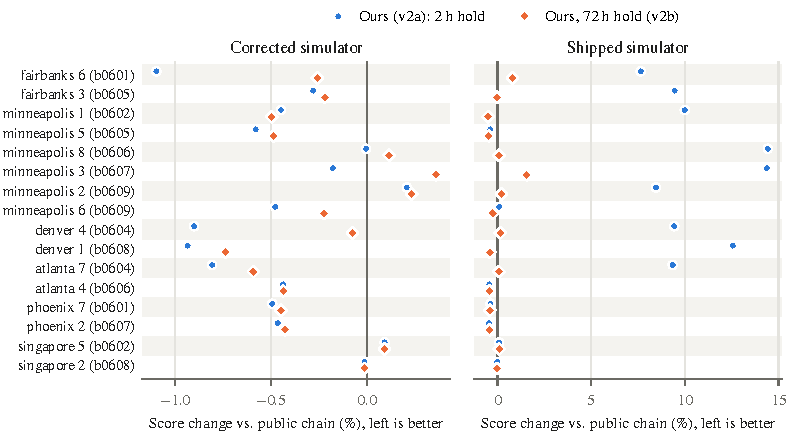
\includegraphics[width=\linewidth]{figures/flip.pdf}
  \caption{Per-scenario change in 30-day score relative to the public chain on val16. On the corrected simulator both variants improve most scenarios; on the shipped simulator the 2-hour hold (v2a) loses 7.6 to 14.4\% in 10 of the 12 cold and mild scenarios, while keeping the 72-hour hold (v2b) stays within 1.6\% everywhere.}
  \label{fig:flip}
\end{figure}

\begin{table}[t]
  \caption{Full 30-day episodes on the 16 held-out val16 scenarios and, in the last block, on the 30 public training scenarios, which we did not use for tuning. Scores and terms are in units of $10^{-3}$ (mean over scenarios of the negated mean per-step reward; lower is better). Cold = Fairbanks, Minneapolis, Denver; mild = Atlanta; hot = Phoenix, Singapore (the public scenarios have no Minneapolis).}
  \label{tab:main}
  \centering
  \small
  \resizebox{\linewidth}{!}{\begin{tabular}{llrrrrr}
\toprule
Controller & Scenarios, simulator & Score & Comfort & Energy & Carbon & Cold / Mild / Hot \\
\midrule
PID + water reset (organizer baseline) & val16, corrected & 43.284 & 29.566 & 7.021 & 6.697 & 51.224 / 28.797 / 30.676 \\
Public chain~\citep{penguin2026} & val16, corrected & 7.464 & 0.433 & 3.349 & 3.682 & 8.898 / 4.993 / 5.116 \\
Public chain, $\lambda_{\mathrm{gas}}=0.5$ (v1) & val16, corrected & 7.464 & 0.433 & 3.349 & 3.682 & 8.897 / 4.993 / 5.116 \\
\rowcolor[HTML]{EDF3FC}Ours, 72 h hold (v2b) & val16, corrected & 7.451 & 0.381 & 3.362 & 3.708 & 8.885 / 4.968 / 5.108 \\
\rowcolor[HTML]{EDF3FC}\textbf{Ours} (v2a) & val16, corrected & 7.444 & 0.382 & 3.360 & 3.702 & 8.875 / 4.964 / 5.107 \\
\midrule
PID + water reset (organizer baseline) & val16, shipped & 40.252 & 28.391 & 6.190 & 5.671 & 46.368 / 28.863 / 30.657 \\
Public chain~\citep{penguin2026} & val16, shipped & 7.442 & 0.425 & 3.342 & 3.676 & 8.855 / 5.011 / 5.124 \\
\rowcolor[HTML]{EDF3FC}Ours, 72 h hold (v2b) & val16, shipped & 7.436 & 0.376 & 3.355 & 3.705 & 8.852 / 4.998 / 5.116 \\
\rowcolor[HTML]{EDF3FC}\textbf{Ours} (v2a) & val16, shipped & 7.973 & 0.456 & 3.470 & 4.047 & 9.676 / 5.168 / 5.117 \\
\midrule
Public chain~\citep{penguin2026} & public 30, corrected & 6.885 & 0.178 & 3.547 & 3.160 & 8.937 / 4.334 / 6.109 \\
\rowcolor[HTML]{EDF3FC}\textbf{Ours} (v2a) & public 30, corrected & 6.915 & 0.140 & 3.593 & 3.183 & 8.919 / 4.316 / 6.211 \\
\bottomrule
\end{tabular}}
\end{table}

\paragraph{Ablations.} Table~\ref{tab:ablate} varies one component at a time on 10-day episodes (2880 steps) of every val16 scenario. Appendix Table~\ref{tab:chain} gives the contribution of each stage of the public chain itself: together the stages cut the base controller's score by 8.0\%. Since all of our variants include $\lambda_{\mathrm{gas}}=0.5$, we pair them against the public chain with that single change. \emph{Cost weights.} Raising $\lambda_{\mathrm{gas}}$ from 0.30 to 0.50 changes the 10-day score by 0.002\%; over full 30-day episodes it changes 10 of 16 scenarios, none by more than 0.05\%, and doubling the comfort price leaves 8 of 16 scenarios bit-identical and moves none by more than 0.03\%. A decision probe agrees: over 19{,}872 AHU decisions on four val16 scenarios (three days each, 4{,}210 decisions with reheat active), re-solving each decision with $\lambda_{\mathrm{gas}} \in \{0.3, 1.0\}$ or with twice the comfort price changed the chosen action zero times; $\lambda_{\mathrm{gas}}=0$ changed 5.9\% of decisions in one cold scenario and a quarter of the comfort price 0.02\% in two. \emph{Comfort band.} Both halving and doubling the 0.08\,K comfort margin make the score worse, and raising the night and weekend floor from 274\,K to a frost-protection 280\,K costs 1.2\%. The 303\,K cooling ceiling changes only three scenarios, all for the better ($-0.15\%$), but costs up to 4.9\% in the highest-load public Phoenix episodes (see Held-out results); 300\,K is worse. \emph{Start-up.} The 0.05\,h/K rule is the largest single gain we found, $-0.44\%$ (interval $-0.68$ to $-0.27\%$) with 13 of 16 scenarios improving. Most of this gain does not come from starting earlier: applying the rule only more than one hour before comfort hours gives $-0.10\%$ and changes just three scenarios, so the rest comes from holding the full comfort margin inside the flag hour; over the 10-day screens the rule changed the band in 12{,}961 zone-steps inside the flag hour and in only 92 earlier ones, all in three cold scenarios. Steeper leads remove more comfort regret but cost more energy and carbon than they save: with $\ell_0=0.5$\,h, $\ell_1=0.35$\,h/K and a 10\,h cap, comfort regret falls from 0.38 to $0.06\times10^{-3}$ while energy plus carbon rises from 7.05 to $7.99\times10^{-3}$. \emph{Hot water.} Shortening the post-demand hold from 72 to 2 hours improves the score by 0.14\% on the corrected simulator (interval 0.05 to 0.32\%) but worsens it by 6.2\% on the shipped one (interval 3.8 to 7.6\%, 10 of 16 scenarios worse), consistent with the long hold drawing much of its value from the tank billing artifact. The hot-water floor (310 to 335\,K) changes the score by at most 0.04\%. \emph{Combined.} The three changes give $-0.71\%$ on the 10-day screens (interval $-1.20$ to $-0.44\%$, 14 of 16 better); keeping the 72-hour hold gives $-0.57\%$. On the shipped simulator the same pair gives $+6.58\%$ and $-0.46\%$: there the shorter hold is the only change that loses.

\begin{table}[t]
  \caption{Ablations on 10-day val16 episodes, scores in $10^{-3}$; negative $\Delta$ is better. Each block is paired against its reference run (reference score in parentheses). ``Better / 16'' counts scenarios that improve; ``tied'' means within $10^{-9}$. Oracle rows read the simulator's internal occupancy model and are not admissible controllers.}
  \label{tab:ablate}
  \centering
  \small
  \resizebox{\linewidth}{!}{\begin{tabular}{lrrr}
\toprule
Variant (10-day val16) & Score & $\Delta$ vs.\ ref. & Better / 16 \\
\midrule
\multicolumn{4}{l}{\emph{Corrected simulator: cost weight, ref.\ public chain} (ref.\ 7.436)} \\
Gas price $\lambda_{\mathrm{gas}}$ 0.30 $\to$ 0.50 & 7.436 & +0.00\% & 4 (9 tied) \\
\midrule
\multicolumn{4}{l}{\emph{Corrected simulator: our changes, ref.\ public chain with $\lambda_{\mathrm{gas}}=0.5$} (ref.\ 7.436)} \\
Comfort margin 0.08 $\to$ 0.04 K & 7.470 & +0.45\% & 0 \\
Comfort margin 0.08 $\to$ 0.16 K & 7.462 & +0.35\% & 2 \\
Standby floor 274 $\to$ 280 K (frost limit) & 7.523 & +1.17\% & 0 (12 tied) \\
Standby ceiling 307 $\to$ 303 K & 7.425 & $-$0.15\% & 3 (13 tied) \\
Standby ceiling 307 $\to$ 300 K & 7.465 & +0.39\% & 2 (9 tied) \\
Pre-conditioning ramp 1 $\to$ 0.5 h & 7.474 & +0.51\% & 3 \\
Water hold after demand 72 $\to$ 12 h & 7.429 & $-$0.09\% & 10 (4 tied) \\
Water hold after demand 72 $\to$ 2 h & 7.426 & $-$0.14\% & 9 (4 tied) \\
Water reservoir floor 320 $\to$ 310 K & 7.436 & $-$0.01\% & 1 (15 tied) \\
Water reservoir floor 320 $\to$ 335 K & 7.439 & +0.04\% & 1 (13 tied) \\
Opt.\ start $\ell_0$ 0.5 h, $\ell_1$ 0.35 h/K, cap 10 h & 8.053 & +8.30\% & 4 \\
Opt.\ start $\ell_0$ 0.25 h, $\ell_1$ 0.10 h/K, cap 3 h & 7.449 & +0.17\% & 9 \\
Opt.\ start $\ell_0$ 0.25 h, $\ell_1$ 0.07 h/K, cap 3 h & 7.426 & $-$0.13\% & 12 \\
Opt.\ start $\ell_0$ 0.25 h, $\ell_1$ 0.05 h/K, cap 3 h & 7.404 & $-$0.44\% & 13 \\
Opt.\ start $\ell_0$ 0.25 h, $\ell_1$ 0.03 h/K, cap 3 h & 7.442 & +0.08\% & 8 \\
Opt.\ start, 0.05 h/K, only $>$1 h before comfort & 7.429 & $-$0.10\% & 2 (13 tied) \\
Ceiling 303 K + 12 h hold & 7.418 & $-$0.25\% & 12 (2 tied) \\
Ceiling 303 K + 2 h hold & 7.414 & $-$0.29\% & 11 (2 tied) \\
\rowcolor[HTML]{EDF3FC}\textbf{Ours} (v2a): opt.\ start 0.05 h/K + ceiling 303 K + 2 h hold & 7.383 & $-$0.71\% & 14 \\
\rowcolor[HTML]{EDF3FC}Ours, keeping the 72 h hold (v2b) & 7.394 & $-$0.57\% & 13 \\
Oracle: per-zone departures (relax empty zones after 13:00) & 7.050 & $-$5.20\% & 16 \\
\midrule
\multicolumn{4}{l}{\emph{Corrected simulator: occupancy oracle, ref.\ public chain} (ref.\ 7.436)} \\
Schedule-only control with the oracle's band formula & 7.726 & +3.90\% & 3 \\
Oracle: future per-zone occupancy, same band formula & 6.930 & $-$6.81\% & 15 \\
\midrule
\multicolumn{4}{l}{\emph{Shipped simulator, ref.\ public chain with $\lambda_{\mathrm{gas}}=0.5$} (ref.\ 7.455)} \\
Water hold after demand 72 $\to$ 2 h & 7.918 & +6.21\% & 2 (4 tied) \\
\rowcolor[HTML]{EDF3FC}Ours, keeping the 72 h hold (v2b) & 7.421 & $-$0.46\% & 13 \\
\rowcolor[HTML]{EDF3FC}\textbf{Ours} (v2a) & 7.946 & +6.58\% & 5 \\
\bottomrule
\end{tabular}}
\end{table}

\paragraph{The value of occupancy information.} The comfort term is weighted by the occupants present in each zone, who arrive in the morning and leave in the afternoon at random times; the observation exposes only the building-wide head count. Two analysis-only oracles read the simulator's per-zone occupancy. The first relaxes a zone to the standby band after 13:00 once the zone has been occupied that day and is now empty; it improves the 10-day score by 5.2\% and wins on all 16 scenarios. The second knows each zone's future occupancy, pre-conditions one hour before each zone's first arrival and idles empty zones. It also replaces the base band formula, so we pair it with a schedule-only control that uses the same formula with the published comfort schedule. The oracle improves on the public chain by 6.8\% and on that control by 10.3\% (interval 5.4 to 16.5\%); the control itself is 3.9\% worse than the public chain, because the rebuilt formula drops the chain's error-scaled margin and empty-day logic. On one 30-day Fairbanks episode the same oracle gains only 2.0\% on the corrected simulator and 0.05\% on the shipped one, so in that cold episode the information is worth much less than on the val16 screens. These are gains of particular hand-designed uses of the information, not upper bounds.

The simulator adds 70\,W of sensible heat per occupant to that occupant's zone, so we tested whether the controller's model sees it. We logged the controller's exponentially smoothed per-zone residual, converted to an implied disturbance power, next to the true occupancy over four days in four val16 scenarios. During working hours the median (across zones) standard deviation of that power is 450 to 690\,W, against an expected signal of 70 to 140\,W for the one to two occupants of an occupied zone. In an event study over 45 to 74 afternoon departures per scenario, the median change in implied power from the half hour before a departure to 15 to 40 minutes after it is between $-33$ and $+67$\,W rather than the expected drop, and occupied zones show lower implied power than empty ones ($-156$ to $-409$\,W), which points to time-of-day confounding in the residual. Our test therefore detects no occupant heat. A dedicated estimator using raw, delay-aligned one-step errors and the building head count might do better, so this is a negative result for this estimator only.

\paragraph{What the development leaderboard rewards.} Two artifacts of the development simulator were discussed publicly: the tank billing artifact (Section~\ref{sec:protocol}), and a fixed random seed in the occupancy model, so replaying the model yields the future-occupancy information of our second oracle. The organizers have banned seed replay and will use a new seed in the final round. Table~\ref{tab:exploit} measures both on seven-day episodes of public building building\_train\_8 in five climates. The sawtooth rule charges the tank to 350\,K whenever there is hot-water demand and the tank is below 330\,K, keeps charging until the tank reaches 349.5\,K, and otherwise commands 310\,K. On the shipped simulator it gains 7.2\%, and combined with future occupancy 15.4\%; on the corrected simulator the sawtooth gains 0.3\%. In one 30-day Fairbanks episode the sawtooth alone gains 22.5\% on the shipped simulator and loses 1.7\% on the corrected one. Applying the seven-day combined gain naively to the public chain notebook's leaderboard score (0.00988) would move it to about 0.0084, roughly 29\% of the way to the top entry (0.00459). This naive extrapolation says nothing about any particular entry; it only shows that part of the development-leaderboard spread need not reflect physically consistent control.

\begin{table}[t]
  \caption{Simulator-artifact accounting: seven-day episodes of building\_train\_8 in five climates, scores in $10^{-3}$. Gains are relative to the public chain on the same simulator; positive gain is better.}
  \label{tab:exploit}
  \centering
  \small
  \begin{tabular}{lrrrr}
\toprule
 & \multicolumn{2}{c}{Shipped simulator} & \multicolumn{2}{c}{Corrected simulator} \\
Policy & Score & Gain & Score & Gain \\
\midrule
Public chain & 7.376 & -- & 7.239 & -- \\
+ tank sawtooth & 6.844 & +7.2\% & 7.214 & +0.3\% \\
+ future occupancy (oracle) & 6.974 & +5.5\% & 6.902 & +4.7\% \\
+ sawtooth and future occupancy & 6.237 & +15.4\% & 6.815 & +5.8\% \\
\bottomrule
\end{tabular}
\end{table}

\section{Limitations}
val16 has 16 scenarios from 8 buildings, so differences below a few tenths of a percent are within building-to-building variation, and small ablation effects are directional. Rescaling the generator's footprints into the public size range is our assumption about the hidden buildings, motivated by the nine-hour runtime limit, and five of the six val16 stations are public stations in new months, whereas leaderboard stations are unseen. The corrected simulator is built from two open community pull requests, not from the organizers' final commit, and the final round may change more. Ablations use 10-day episodes from each strip's start date, which under-sample late-month weather. The artifact measurements use one public building and a hand-written sawtooth rule. We tuned four parameters on val16 itself (the start-up lead and its cap, the cooling ceiling and the hold time), so val16 numbers for our final controller are optimistic. Our out-of-sample check on the public training buildings, on which the public chain was itself developed, shows the cost: there the full set of changes is 0.44\% worse than the public chain, because val16's two Phoenix episodes are milder than the three highest-load public ones and let a weather-dependent change through.

\section{Conclusion}
On held-out buildings with corrected physics, the strongest public controller we found leaves little room within the information it observes. Its cost weights barely influence its decisions. The largest lever we identified is per-zone occupancy, where our oracles gain 5 to 7\% over the public chain, but our test found no usable trace of occupant heat in the controller's model residual. The improvements that survive are small: sharper start-up before occupancy and a 2-hour hot-water hold instead of a 72-hour one improve the public scenarios by only 0.19\%, with an interval that crosses zero. A lower unoccupied cooling ceiling that helped on val16 cost up to 4.9\% in the highest-load public episodes. The 72-hour hold, worth 6.2\% on the shipped simulator and slightly harmful after the fix, shows how simulator artifacts can shape tuning. We release our protocol, patches and per-scenario results so that others can check their controllers the same way.

\begin{ack}
We thank the challenge organizers and the participants who publicly shared controllers and simulator analyses. This work received no external funding.
\end{ack}

\bibliographystyle{plainnat}
\bibliography{references}

\clearpage
\appendix
\section{Validation scenarios}
\label{app:val16}
\begin{table}[!h]
  \caption{val16: generated buildings (seeds 601, 602, 604 to 609; seeds 600 and 603 fail the generator's minimum-zone check after rescaling) and their weather strips.}
  \centering
  \small
  \begin{tabular}{lrrl}
\toprule
Building & AHUs & Zones & Weather strips \\
\midrule
building\_0601 & 6 & 43 & fairbanks\_6, phoenix\_7 \\
building\_0602 & 6 & 24 & minneapolis\_1, singapore\_5 \\
building\_0604 & 5 & 19 & atlanta\_7, denver\_4 \\
building\_0605 & 6 & 29 & fairbanks\_3, minneapolis\_5 \\
building\_0606 & 6 & 34 & atlanta\_4, minneapolis\_8 \\
building\_0607 & 5 & 41 & minneapolis\_3, phoenix\_2 \\
building\_0608 & 6 & 19 & denver\_1, singapore\_2 \\
building\_0609 & 4 & 35 & minneapolis\_2, minneapolis\_6 \\
\bottomrule
\end{tabular}
\end{table}

\section{Stages of the public chain}
\begin{table}[!h]
  \caption{Cumulative stages of the public controller chain on 10-day val16 episodes, corrected simulator, paired against the full chain; scores in $10^{-3}$.}
  \label{tab:chain}
  \centering
  \small
  \begin{tabular}{lrrr}
\toprule
Variant (10-day val16) & Score & $\Delta$ vs.\ ref. & Better / 16 \\
\midrule
\multicolumn{4}{l}{\emph{Corrected simulator: public chain components, ref.\ public chain} (ref.\ 7.436)} \\
Base MPC only~\citep{wu2026cpu} & 8.079 & +8.65\% & 0 \\
+ error reserve & 8.058 & +8.37\% & 0 \\
+ identified response gain, 36 h warm-water standby & 7.887 & +6.06\% & 1 \\
+ 72 h hold, 274 K setback, fast recovery & 7.688 & +3.38\% & 2 \\
+ empty-day relaxation, 0.5 K SAT grid, error-scaled margin & 7.506 & +0.94\% & 3 (4 tied) \\
+ demand-sized water temperature (320 K floor) & 7.437 & +0.01\% & 2 (5 tied) \\
\bottomrule
\end{tabular}
\end{table}

\end{document}
